% The corpus's synthetic PGF page: the backend's shading, soft-mask and tiling-pattern paths (dlist.md), which arXiv
% papers in the corpus rarely reach. One feature per row, labelled.
\documentclass[11pt]{article}
\usepackage[margin=1in]{geometry}
\usepackage{tikz}
\usetikzlibrary{fadings,patterns,shadings}
\pagestyle{empty}
\begin{document}
\section*{Shadings}
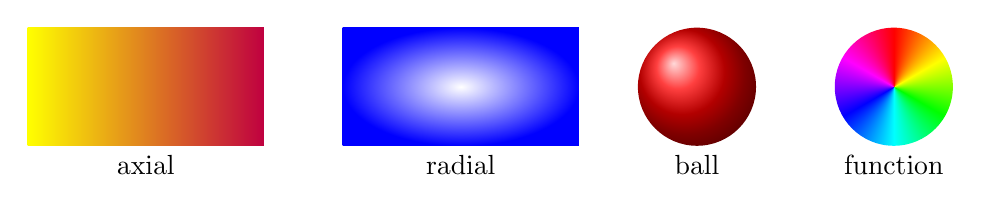
\begin{tikzpicture}
  \shade[left color=yellow, right color=purple] (0,0) rectangle (3,1.5);              \node[below] at (1.5,0) {axial};
  \shade[inner color=white, outer color=blue] (4,0) rectangle (7,1.5);                \node[below] at (5.5,0) {radial};
  \shade[ball color=red] (8.5,0.75) circle (0.75);                                    \node[below] at (8.5,0) {ball};
  \shade[shading=color wheel] (11,0.75) circle (0.75);                                \node[below] at (11,0) {function};
\end{tikzpicture}

\section*{Soft masks (fadings)}
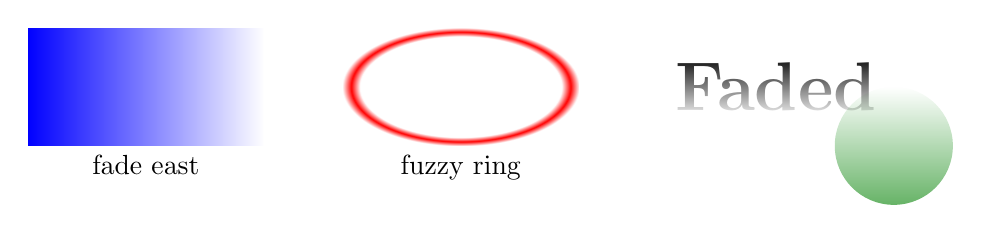
\begin{tikzpicture}
  \fill[blue, path fading=east] (0,0) rectangle (3,1.5);                              \node[below] at (1.5,0) {fade east};
  \fill[red, path fading=fuzzy ring 15 percent] (4,0) rectangle (7,1.5);              \node[below] at (5.5,0) {fuzzy ring};
  \node[font=\Huge\bfseries, scope fading=south] at (9.5,0.75) {Faded};
  \fill[green!50!black, opacity=0.6, path fading=north] (11,0) circle (0.75);
\end{tikzpicture}

\section*{Tiling patterns}
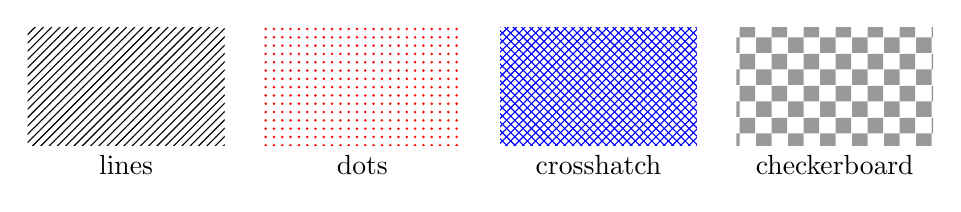
\begin{tikzpicture}
  \fill[pattern=north east lines] (0,0) rectangle (2.5,1.5);                          \node[below] at (1.25,0) {lines};
  \fill[pattern=dots, pattern color=red] (3,0) rectangle (5.5,1.5);                   \node[below] at (4.25,0) {dots};
  \fill[pattern=crosshatch, pattern color=blue] (6,0) rectangle (8.5,1.5);            \node[below] at (7.25,0) {crosshatch};
  \fill[pattern=checkerboard, pattern color=black!40] (9,0) rectangle (11.5,1.5);     \node[below] at (10.25,0) {checkerboard};
\end{tikzpicture}

\section*{Blend modes and groups}
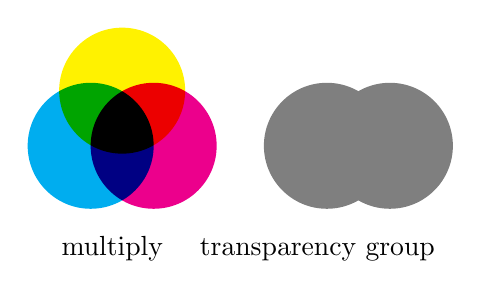
\begin{tikzpicture}
  \begin{scope}[blend group=multiply]
    \fill[cyan] (0,0) circle (0.8); \fill[magenta] (0.8,0) circle (0.8); \fill[yellow] (0.4,0.7) circle (0.8);
  \end{scope}
  \begin{scope}[transparency group, opacity=0.5]
    \fill[black] (3,0) circle (0.8); \fill[black] (3.8,0) circle (0.8);
  \end{scope}
  \node at (2,-1.3) {multiply \quad transparency group};
\end{tikzpicture}
\end{document}
